\section{State and explain the Latka-Volterra predator prey model}
\section*{Also find the exact solution and make a stability analysis and sketch the phase portrait of the population dynamics}
\subsection*{ Statement and Explanation of the Model}

Let $x(t)$ denote the prey population density and $y(t)$ denote the predator population density at time $t$. The classic Lotka--Volterra system is defined by:

\begin{align*}
    \frac{dx}{dt} &= \alpha x - \beta xy \sidenote{1} \\
    \frac{dy}{dt} &= -\gamma y + \delta xy \sidenote{2}
\end{align*}
where parameters $\alpha, \beta, \gamma, \delta > 0$.

\vspace{0.5em}
\begin{itemize}
    \item $\alpha x$: Exponential growth of prey in the absence of predators.
    \item $-\beta xy$: Rate of prey mortality due to predation (proportional to interaction frequency).
    \item $-\gamma y$: Exponential death/decay rate of predators in the absence of prey.
    \item $\delta xy$: Rate of predator population increase resulting from consuming prey.
\end{itemize}

\vspace{1em}
\noindent\textbf{Explanation:}

\noindent From the prey equation, we observe that in the absence of predators, the prey population increases without limit, and in the presence of predators, the growth rate of the prey population is reduced by an amount proportional to the predator population present.

\vspace{0.5em}
\noindent Similarly, from the predator equation, we find that in the absence of prey, the predator population decreases and becomes extinct due to starvation; and in the presence of the prey population, the growth rate of the predator population is increased by an amount proportional to the prey population present.
\subsection*{Exact Solution}

\noindent The model (1) can be written as:
\begin{align*}
    \frac{dy}{dx} &= \frac{y(-\gamma + \delta x)}{x(\alpha - \beta y)} \\
    \Rightarrow \frac{dy}{dx} &= \frac{xy\left(-\frac{\gamma}{x} + \delta\right)}{xy\left(\frac{\alpha}{y} - \beta\right)} \\
    \Rightarrow \frac{dy}{dx} &= \frac{\delta - \frac{\gamma}{x}}{\frac{\alpha}{y} - \beta} \\
    \Rightarrow \left(\frac{\alpha}{y} - \beta\right) dy &= \left(\delta - \frac{\gamma}{x}\right) dx \sidenote{separating variables} \\
    \Rightarrow \alpha \frac{dy}{y} - \beta \, dy &= \delta \, dx - \gamma \frac{dx}{x}
\end{align*}

\noindent Integrating, we get:
\begin{align*}
    \alpha \ln y - \beta y &= \delta x - \gamma \ln x + \ln k \sidenote{by integrating} \\
    \Rightarrow \ln y^\alpha - \ln e^{\beta y} &= \ln e^{\delta x} - \ln x^\gamma + \ln k \\
    \Rightarrow \ln y^\alpha - \ln e^{\beta y} - \ln e^{\delta x} + \ln x^\gamma &= \ln k \\
    \Rightarrow \ln \frac{y^\alpha}{e^{\beta y}} + \ln \frac{x^\gamma}{e^{\delta x}} &= \ln k \\
    \Rightarrow \ln \frac{x^\gamma y^\alpha}{e^{\delta x} e^{\beta y}} &= \ln k \\
    \Rightarrow \frac{x^\gamma y^\alpha}{e^{\delta x + \beta y}} &= k \sidenote{II}
\end{align*}

where $k$ is the integral constant, which is the \textbf{general solution}.

\vspace{1em}
\noindent Using initial conditions $x(0) = x_0$ and $y(0) = y_0$, we get:
\begin{align*}
    \frac{x_0^\gamma y_0^\alpha}{e^{\delta x_0} e^{\beta y_0}} &= k
\end{align*}

\noindent Putting the value of $k$ in (II), we get:
\begin{align*}
    \frac{x^\gamma y^\alpha}{e^{\delta x} e^{\beta y}} &= \frac{x_0^\gamma y_0^\alpha}{e^{\delta x_0} e^{\beta y_0}} \sidenote{III}
\end{align*}
which is the \textbf{particular solution} of (1).

\vspace{1em}
\noindent Using $f(x) = \frac{x^\gamma}{e^{\delta x}}$ and $g(y) = \frac{y^\alpha}{e^{\beta y}}$:
\begin{align*}
    \therefore f(x) \cdot g(y) &= K \sidenote{IV}
\end{align*}
\subsection*{ Extrema Analysis for $f(x)$}

From (IV), it is observed that $f(x)$ and $g(y)$ are inversely related.

\vspace{0.5em}
\noindent Also, $f(0) = 0$ when $x = 0$, and $f(x) \to 0$ as $x \to \infty$.

\vspace{1em}
\noindent Now,
\begin{align*}
    \frac{df}{dx} &= (\gamma - \delta x) x^{\gamma - 1} e^{-\delta x}
\end{align*}

\noindent and
\begin{align*}
    \frac{d^2 f}{dx^2} &= \left[(\gamma - \delta x)^2 - \gamma \right] x^{\gamma - 2} e^{-\delta x}
\end{align*}

\noindent For optimum value, $\frac{df}{dx} = 0$:
\begin{align*}
    \therefore (\gamma - \delta x) x^{\gamma - 1} e^{-\delta x} = 0 \implies x = \frac{\gamma}{\delta}
\end{align*}

\noindent Now for $x = \frac{\gamma}{\delta}$:
\begin{align*}
    \frac{d^2 f}{dx^2} &= \left[(\gamma - \gamma)^2 - \gamma\right] \left(\frac{\gamma}{\delta}\right)^{\gamma - 2} e^{-\gamma} = -\gamma \left(\frac{\gamma}{\delta}\right)^{\gamma - 2} e^{-\gamma} \\
    \therefore \frac{d^2 f}{dx^2} &< 0
\end{align*}

\vspace{0.5em}
\noindent Hence, $f(x)$ has a \textbf{local maximum} at $x = \frac{\gamma}{\delta}$.\\
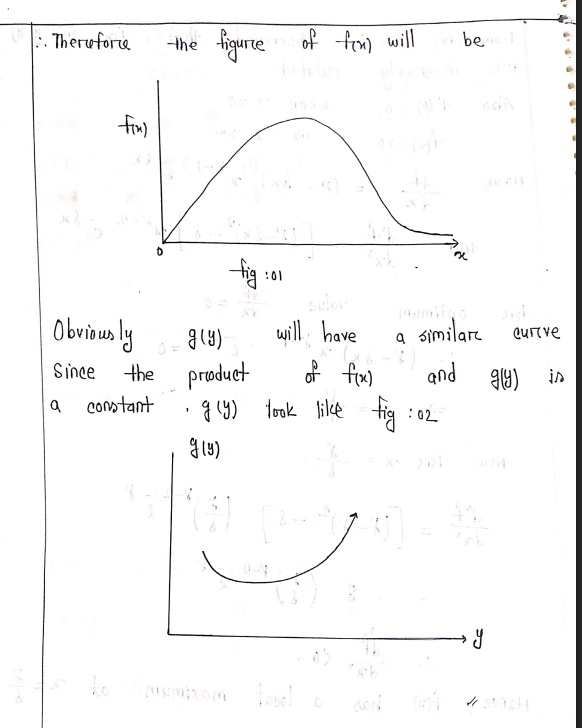
\includegraphics[]{Image/Lotka volterra1.png}
\subsection*{Stability Analysis}

System (i) cannot be solved to find $x(t)$ and $y(t)$ explicitly, so the exact path of (i) cannot be drawn. We look for points where the population remains constant (for an indefinite time) and find the paths of (i) in the neighborhood of these equilibrium points.

\vspace{0.5em}
\noindent The equilibrium points of (i) are given by:
\begin{align*}
    \left.
    \begin{aligned}
        x(\alpha - \beta y) &= 0 \\
        y(-\gamma + \delta x) &= 0
    \end{aligned}
    \right\} \sidenote{v}
\end{align*}

\noindent Solving (v), we find the equilibrium points $A(0, 0)$ and $B\left(\frac{\gamma}{\delta}, \frac{\alpha}{\beta}\right)$.

\vspace{0.5em}
\noindent We note that these are also solutions of (i) which are independent of time and can be considered as special cases in which the curves degenerate into points.

\vspace{0.5em}
\noindent We now investigate the stability of $A(0, 0)$ and $B\left(\frac{\gamma}{\delta}, \frac{\alpha}{\beta}\right)$.

\vspace{1em}
\noindent\textbf{Case I --- Equilibrium Point $A(0, 0)$:}

\noindent This is the case where both the prey and the predator populations are absent. Thus, when the populations are sufficiently close to this point, we can neglect the second terms $\beta xy$ and $\delta xy$ of (i) in comparison to the first terms. Hence, (i) reduces to:
\begin{align*}
    \left.
    \begin{aligned}
        \frac{dx}{dt} &= \alpha x \\
        \frac{dy}{dt} &= -\gamma y
    \end{aligned}
    \right\} \sidenote{vi}
\end{align*}

\noindent with solutions:
\begin{align*}
    x(t) = c_1 e^{\alpha t} \quad \text{and} \quad y(t) = c_2 e^{-\gamma t} \sidenote{vii}
\end{align*}

where $c_1$ and $c_2$ are arbitrary constants. Since $x$ and $y$ are non-negative, we must have $c_1 \ge 0$, $c_2 \ge 0$, and the family of curves described by (vii) is shown in \textbf{fig: 03}.

\vspace{0.5em}
\noindent Further, if we displace the population slightly from the equilibrium point $(0, 0)$, then it tends to move away from the point $(0, 0)$.
\begin{align*}
    \therefore \text{The equilibrium point } A(0, 0) \text{ is } \textbf{unstable}.
\end{align*}
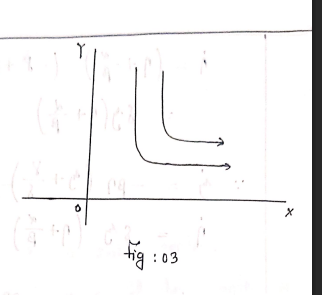
\includegraphics[]{Image/Lotka-volterra3.png}
\subsection*{Case II --- Equilibrium Point $B\left(\frac{\gamma}{\delta}, \frac{\alpha}{\beta}\right)$ Perturbation}

\vspace{0.5em}
\noindent This is the case where both species are present. We consider (i) by using:
\begin{align*}
    \left.
    \begin{aligned}
        x &= \xi + \frac{\gamma}{\delta} \\
        y &= \eta + \frac{\alpha}{\beta}
    \end{aligned}
    \right\} \sidenote{ix}
\end{align*}
\begin{align*}
    \frac{d\xi}{dt} &= \left(\xi + \frac{\gamma}{\delta}\right) (\alpha - \beta\eta - \alpha) = -\beta\eta \left(\xi + \frac{\gamma}{\delta}\right) \\
    \therefore \dot{\xi} &= -\beta\eta \left(\xi + \frac{\gamma}{\delta}\right) \\
    \implies \dot{\xi} &= -\beta\xi\eta - \frac{\gamma\beta}{\delta}\eta \\
   \therefore \text{Similarly}\, \dot{\eta} &= \delta\xi\eta + \frac{\alpha\delta}{\beta}\xi
\end{align*}

\noindent Since $\xi$ and $\eta$ are small, we can neglect the non-linear terms of $\xi\eta$:
\begin{align*}
    \left.
    \begin{aligned}
        \dot{\xi} &= -\frac{\gamma\beta}{\delta} \eta =a\xi + b\eta \\
        \dot{\eta} &= \frac{\alpha\delta}{\beta} \xi=c\xi + d\eta
    \end{aligned}
    \right\} \sidenote{x}
\end{align*}

\noindent Here $a = 0, b = -\frac{\gamma\beta}{\delta}, c = \frac{\alpha\delta}{\beta}, d = 0$.(linearized equation)

\vspace{0.5em}
\noindent $\therefore$ The characteristic equation is:
\begin{align*}
    \lambda^2 - (a + d)\lambda + (ad - bc) = 0
\end{align*}
\begin{align*}
    \implies \lambda^2 - (0 + 0) + \left(0 + \frac{\gamma\beta}{\delta} \cdot \frac{\alpha\delta}{\beta}\right) &= 0 \\
    \implies \lambda^2 &= -\alpha\gamma \\
    \implies \lambda &= \pm \sqrt{-\alpha\gamma} \\
    \therefore \lambda &= \pm i\sqrt{\alpha\gamma}
\end{align*}

\noindent Thus, $B\left(\frac{\gamma}{\delta}, \frac{\alpha}{\beta}\right)$ is a \textbf{stable center}(Eigen value is purely imaginary).
\noindent To know the exact shape of the center, we eliminate $t$ from (x) and obtain:
\begin{align*}
    \frac{d\xi}{d\eta} &= \frac{-\frac{\gamma\beta}{\delta}\eta}{\frac{\alpha\delta}{\beta}\xi} = -\frac{\gamma\beta}{\delta}\eta \times \frac{\beta}{\alpha\delta\xi} = -\frac{\gamma\beta^2}{\alpha\delta^2} \frac{\eta}{\xi} \\
    \implies \xi \, d\xi &= -\frac{\gamma\beta^2}{\alpha\delta^2} \eta \, d\eta \\
    \implies \frac{1}{\gamma\beta^2} \xi \, d\xi + \frac{1}{\alpha\delta^2} \eta \, d\eta &= 0
\end{align*}

\noindent Integrating, we get:
\begin{align*}
    \frac{1}{\gamma\beta^2} \frac{\xi^2}{2} + \frac{1}{\alpha\delta^2} \frac{\eta^2}{2} &= \frac{c^2}{2} \\
    \implies \frac{\xi^2}{\gamma\beta^2} + \frac{\eta^2}{\alpha\delta^2} &= c^2 \\
    \implies \frac{\xi^2}{\gamma\beta^2 c^2} + \frac{\eta^2}{\alpha\delta^2 c^2} &= 1 \sidenote{xi}
\end{align*}

where $c$ is a constant.

\vspace{0.5em}
\noindent This represents a family of \textbf{concentric ellipses}. We find from (xi) that the directions of the ellipses are \textbf{anti-clockwise}.(eqn x has different sign) Hence, the stable center $B\left(\frac{\gamma}{\delta}, \frac{\alpha}{\beta}\right)$ is shown in \textbf{fig: 04}.
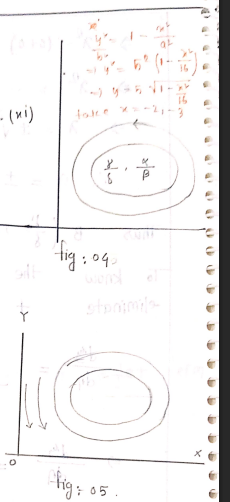
\includegraphics[]{Image/Lotka4.png}

\vspace{0.5em}
\noindent From \textbf{fig: 01}, it is clear that for any value of $f(x)$, there are either two values of $x$ or none. Same arguments hold for $y$ also. This implies that the path of (i) is a \textbf{closed loop} as shown in \textbf{fig: 05}.

\vspace{0.5em}
\noindent Hence, from \textbf{fig: 03}, \textbf{fig: 04}, and \textbf{fig: 05}, the population dynamics of (i) near its equilibrium points are shown in the phase plane.